\documentclass[parskip=half]{scrartcl}
\usepackage[utf8]{inputenc}
\usepackage{siunitx}
\DeclareSIUnit\year{y}
\DeclareSIUnit\kWhr{kWh}
\DeclareSIUnit\MWh{MWh}
\DeclareSIUnit\GBP{£}
\DeclareSIUnit\bar{bar}
\DeclareSIUnit\pence{p}

\usepackage{comment}
\usepackage{amsmath}
\usepackage{graphicx}

\usepackage[
backend=biber,
style=authoryear,
sorting=ynt
]{biblatex} % needed for citations and references
\usepackage{csquotes} % recommended for use with biblatex
\usepackage{xpatch} % recommended for use with biblatex
\addbibresource{references.bib} % name of the references file

\usepackage{hyperref}
\hypersetup{
    colorlinks=true,
    linkcolor=blue,
    filecolor=magenta,      
    urlcolor=cyan,
} % style of the hyperlinks
\urlstyle{same}
\usepackage{cleveref}

\title{A Community District Heating Scheme}
\author{}
\date{}

\begin{document}

\maketitle
\section{Introduction}

\begin{figure}[ht]\label{fig1}
\centering
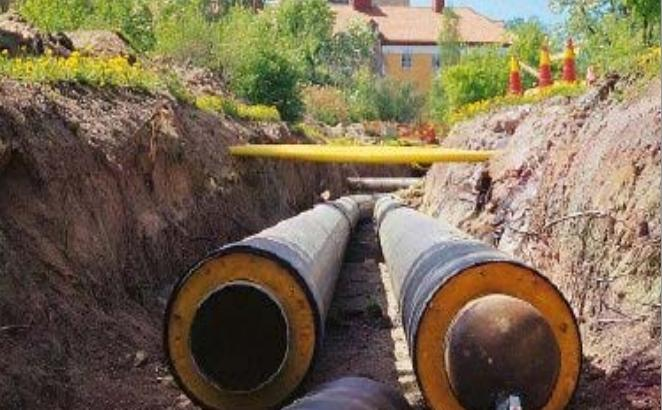
\includegraphics[width=0.8\textwidth]{HeatMain.jpg}
\caption{An insulated  flow-pipe and return-pipe pair to be used in a district heating network}
\end{figure}
    
District Heat Networks (DHNs) are as seen in Figure \ref{fig1} are widely used in parts of Europe, especially in cities. They provide 36\% of the heat in Vienna, for example, and in Copenhagen the network extends more than 40 km across the city. 

The central idea is that heat is provided to the network by one or a few large power stations that can be more efficient than individual boilers located at each of the end users. They can also enable heat to be used that would otherwise be wasted, such as from waste to energy plants or geothermal plants.

Normally, hot water is delivered into the main in a flow pipe at temperatures between \SI{90}{\celsius} and \SI{120}{\celsius} and returned from it in a return pipe after heat has been extracted at between \SI{40}{\celsius} to \SI{70}{\celsius}. The pipes themselves are normally steel, polyetyhylene or polybutylene, insulated with PUR foam and covered with high density polyethylene.They are often laid in a trench, in sand, to reduce expanse. Heat is transferred from the main to individual buildings via branch pipes and heat exchangers, and the heating system in the buildings is just as it would normally be.

In this session we will investigate the provision of heat for a community through the use of a central biomass boiler which delivers heat via a district heating system.Your task is to assess the financial and technical details of the scheme.

\SI{24}{\kWhr\per\metre\squared}

\section{The Community}

The community comprises :
\begin{itemize}
\item A block of 4 apartments, total area \SI{240}{\metre\squared}.
\item 3 terraces, each of 8 homes, built in the 1880s.
\item 3 pairs of 1930's semi-detached houses
\item 10 detached Edwardian stone houses.
\item Recreation rooms (eg community centre, village hall etc), of total area \SI{200}{\metre\squared}.
\item A corner shop, area \SI{50}{\metre\squared}.
\end{itemize}

Further details:
\begin{itemize}
\item The space heating and hot water usage of these buildings is variable, depending on the type, but averages out to about \SI{288}{\kWhr\per\metre\squared\per\year} for space heating and \SI{25}{\kWhr\per\metre\squared\per\year} for hot water. The total floor area of the buildings is \SI{7134}{\metre\squared}.

\item The average Heat Loss Parameter (HLP) for the buildings in the community is \SI{5}{\watt\per\kelvin\per\metre\squared}. This is high, indicating that the buildings are not very well insulated. The outside temperature that is exceeded 99\% of the time, $T_{99}$, is \SI{0}{\celsius} and the inside temperature,$T_\text{design}$, of all the buildings is \SI{20}{\celsius}. Water is heated for 25\% of the time.

\item An analysis of demand data for communities like this one suggests that the optimum biomass boiler to install would be one that can meet 70\% peak heat demand. It will cost £800 per kW installed. A replacement gas boiler would have cost £400 per kW installed.

\item It will cost £7000 per dwelling, and a further £25,000 for the recreation and retail spaces to equip them for a district heat main.

\item The heat distribution network consists of a "heat main", which is a large diameter insulated pipe that takes water out from the boiler at \SI{120}{\celsius} and \SI{16}{\bar}, and returns it at \SI{70}{\celsius}. Each house then draws from this heat main via a smaller diameter branch pipe, which delivers heat to its wet plumbing system via a heat exchanger.

\item The heat main pipe is insulated with \SI{50}{\milli\metre} of PIR insulation of thermal conductivity \SI{0.023}{\watt\per\kelvin\per\metre} and is buried underground at an ambient temperature of \SI{12}{\celsius}.

\item The rate of temperature fall with distsance $x$ along the heat main is given by:
\begin{equation}
\label{eq:tfall}
\frac{\delta T}{\delta x}=\frac{4U\Delta T}{\rho c D v}
\end{equation}
where $U$ is the $U$-value of the pipe insulation; $\Delta T$ is the temperature difference between the water in the pipe and the ground outside it; $\rho$ is the density of water = \SI{1000}{\kg\per\metre\cubed}; $c$ is the specific heat capacity of water = \SI{4200}{\joule\per\kg\per\kelvin}; $D$ is the diameter of the pipe and $v$ is the flow speed of the water.

\item The biomass boiler has in addition two accumulator tanks which each hold \SI{12000}{\litre} of hot water at  \SI{120}{\celsius} and 16 bar.

\item The wood chip used has an energy density of \SI{18.0}{\giga\joule} per dry tonne and is 30\% moisture.

\item The boiler is 85\% efficient. 

\item The wood chip costs £100 per tonne delivered.

\item The Renewable Heat Incentive (RHI) scheme may apply to this project. The eligibility criteria for non-domestic RHI are set out by \href{https://www.ofgem.gov.uk/environmental-programmes/non-domestic-renewable-heat-incentive-rhi/eligibility-non-domestic-rhi}{ofgem} (\cite{ofgem}), but also keep an eye out for \href{https://www.gov.uk/government/policies/increasing-the-use-of-low-carbon-technologies/supporting-pages/renewable-heat-incentive-rhi}{DECC's} latest news on the subject. An RHI calculator from the \href{http://www.biomassenergycentre.org.uk/portal/page?_pageid=73,1&_dad=portal&_schema=PORTAL}{Biomass Energy Centre} is available from their home page, on the module and in \href{https://docs.google.com/spreadsheet/ccc?key=0AnLADLTFXDf5dENTeWEydV9OZXZaVk4zV09zcWFnLVE&usp=drive_web#gid=0}{Google Docs}.

\item The wood chip is delivered from a local saw mill 10 km away and the energy cost of deliveries is 1 kWh per tonne km.
\end{itemize}


\section{Questions}
\begin{enumerate}
\item Estimate the annual heat demand, for both hot water and space heating.
\item Given a maximum temperature difference between inside and outside of \SI{20}{\celsius}, estimate the peak power demand for heat, assuming that all properties require water heating at the same time for 6 hours a day.
\item Estimate the size of the boiler required and the purchase cost. 
\item Estimate the total capital cost of the project.
\item What volume flow rate is required in the heat main at periods of maximum heat demand?
\item If the heat main has a diameter of 200 mm, what flow speed does the water have at full capacity?
\item What is the U-value of the insulating layer?
\item Assuming an average water temperature in the main of \SI{95}{\celsius}, what is the temperature fall of the water per 100 m of pipe?
\item What is the purpose of the accumulator tanks in times of (a) peak load and (b) low use?
\item What mass of wood chip is required per year?
\item What is the cost of the wood chip per delivered kWh of heat?
\item What is the annual cost of the wood chip?
\item What is this as a fraction of the capital cost of the project?
\item What is the annual RHI revenue for the scheme?
\item What is the annual energy cost of wood chip delivery?
\item What is this as a fraction of the delivered energy?
\end{enumerate}

%\begin{comment}
\section{Solutions}

\begin{enumerate}
\item One way in which the likely annual space heating demand of these buildings can be found is to start with their collective (average)  heat loss parameter of \SI{5}{\watt\per\kelvin\per\metre\squared}. This, multiplied by the total floor area (TFA) of \SI{7134}{\metre\squared} gives the heat loss coefficient (HLC) for the buildings, which is \SI{35.67}{\kilo\watt\per\kelvin}. This means that the heating system for the set of buildings has to supply an extra \SI{35.67}{\kilo\watt} for every degree colder the outside temperature becomes.

The annual space heating demand of these buildings depends how cold it is outside. Suppose the buildings are in a location where there are 2400 degree days per year (The \href{http://www.eci.ox.ac.uk/research/energy/degreedays.php}{ECI} tells us that is the value in the UK for places about as far north as Newcastle). In that case the annual space heating demand will be (less any gains, which we ignore here)


\begin{align}
\mathrm{Space\ heating\ demand}&=\mathrm{HLC}\times DD\times\frac{24}{1000}\\&=35.67\times 2400\times\frac{24}{1000}\notag\\&=\SI{2054.6}{\MWh\per\year}\notag
\label{eq:shdemand}
\end{align}

The hot water demand is is \SI{25}{\kWh\per\metre\squared\per\year}, so if we multiply this by the given TFA of \SI{7134}{\metre\squared}, we find an annual water heating demand of \SI{178.4}{\mega\watt}. 
Thus the total heat demand is 2054.6 + 178.4 = \SI{2233}{\MWh\per\year}.

So, the total heat requirement is found to be \SI{2233}{\MWh}, of which \SI{178}{\MWh} is for hot water, while \SI{2054.6}{\MWh} is for space heating. Note that the bulk of the heat demand would be for the ten Edwardian houses - which occupy more than 50\% of the total floor area of \SI{7134}{\metre\squared}.

\item To find the peak space heating power demand we need to find the heat loss coefficient, which is the total heat demand per Kelvin temperature difference, then multiply by the maximum likely temperature difference between inside and outside, ie $T_\text{in} - T_{99} = \SI{20}{\kelvin}$.

\begin{align}
P_\text{max} &=\text{HLP}\times\text{TFA}\times\Delta T_\text{max}\\
&=5\times7134\times 20\notag\\ &=\SI{713}{\kilo\watt}\notag
\label{eq:pmax}
\end{align}


To this we need to add the peak heat demand for hot water. We can only estimate this, but if we assume that all properties heat water for 6 hours per day every day, or 2190 hours per year, then the peak hot water power demand is 179/2190 = \SI{0.082}{\mega\watt} = \SI{82}{\kilo\watt}.
Hence we find that the peak heat power demand is \SI{795}{\kilo\watt}.

\item The boiler size required = 70\% of 795 =\SI{556}{\kilo\watt}, at a cost of $556\times800 = \SI{444800}[\GBP]{}$

\item The total cost to equip dwellings = $44\times 7000=\SI{308000}[\GBP]{}$, plus \SI{25000}[\GBP]{} for the rest, making a total of \SI{333000}[\GBP]{} for equipping the buildings for the heat main. Add this to the cost of the boiler and we get a total capital cost of \SI{777800}[\GBP]{}.

\item If the peak demand is $P_\text{max}$, then we need $P_\mathrm{max}=\dot m c \Delta T$ where $\dot m$ is the mass flow rate of water along the main, $c$ is the  specific heat capacity of water, and $\Delta T$ is the temperature fall of the water along the heat main. But, the mass flow rate is the volume flow rate $V$ multiplied by the water density $\rho$, so we need $P_\mathrm{max}=\rho V c \Delta T$.  Hence the required volume flow rate is given by

\begin{align}
V &=\frac{P_\mathrm{max}}{\rho c \Delta T}\\&=\frac{\num{800000}}{1000\times 4128\times 50}\notag\\&=\SI{3.9e-3}{\metre\cubed\per\second}\notag\\&=\SI{3.9}{\litre\per\second}\notag
\label{eq:vfr}
\end{align}

\item If the heat main has cross sectional area $A=\frac{\pi D^2}{4}=\pi r^2$ and the flow speed is $v$ \si{\metre\per\second}, then a cylinder of fluid of length $v$ m will flow into the heat main each second. The volume $Av$ of this cylinder is the volume flow rate $V$. Hence the flow  velocity is given by

\begin{align}
v &=\dfrac{V}{A}\\&=\dfrac{\num{3.9e-3}}{\pi\times 0.1^2}\notag\\&=\SI{12.4}{\cm\per\second}\notag
\label{eq:flowv}
\end{align}

\item The $U$ value of the insulating jacket is given by

\begin{align}
U &=\dfrac{\lambda}{x}\\&=\dfrac{0.023}{0.05}\notag\\&=\SI{0.46}{\watt\per\kelvin\per\metre\squared}
\label{eq:uvalue}
\end{align}

\item From equation \eqref{eq:tfall},

\begin{align}
\dfrac{\delta T}{\delta x}&=\dfrac{4U\Delta T}{\rho c D v}\\ &=\dfrac{4\cdot 0.46\cdot 83}{1000\cdot 4128\cdot 0.2\cdot 0.124}\notag\\ &=\SI{2.1e-3}{\kelvin\per\metre}\notag\\ &=\SI{2.1}{\kelvin} per \SI{100}{\metre}\notag
\end{align}

Hence under these conditions, the heat loss by conduction will cause the water to cool by only by just over \SI{2}{\kelvin} per km of heat main. Study equation \eqref{eq:tfall} to see what would cause these heat losses to increase or decrease.

\item The accumulator tanks are there to enable the biomass boiler to run at near to its design capacity as often as possible, under which conditions it is more efficient and to allow a smaller capacity boiler unit to be used for the same peak load. This is why, in this exercise, the unit was deliberately undersized. When the demand exceeds the capacity of the boiler, hot water is drawn from the tanks, and in times of low demand, the boiler is kept running at a high level, but part of its output is used to top up the tanks. 

\item The community requires a total of \SI{2233}{\MWh} of heat per year. The boiler is 85\% efficient, so the input energy must be $2233 / 0.85 = \SI{2627}{\MWh}$. The wood chip contains \SI{18}{\giga\joule} per dry tonne, but has 30\% moisture content, so as delivered it contains $0.7\times18= \SI{12.6}{\giga\joule\per\tonne}=\SI{3.5}{\MWh\per\tonne}$. Hence the mass required annually = 2627 / 3.5 = 751 tonne per year.

\item Each tonne of wood costs £100 and delivers \SI{3.5}{\MWh} = \SI{3500}{\kWhr} of heat. The price per delivered \si{\kWhr} is therefore £100/3500 = \SI{2.86}{\pence\per\kWhr}.

\item The wood chip costs £100 per delivered tonne, so the annual cost must be $751\times 100 = \SI{75100}[\GBP]{}$, or \SI{10.52}[\GBP]{\metre\per\squared} of floor space.

\item The capital cost is about \SI{800000}[\GBP]{}, so the annual fuel cost, at these prices, is 9.4\% of the capital cost. Compare this with a domestic gas boiler in poorly insulating houses of the sort in this example, where annual gas usage might be \SI{20000}{\kWhr} at \SI{4.9}{\pence\per\kWhr} (December 2013 prices). This would cost \SI{980}[\GBP]{} per year in fuel bills to run, at about £9.80 m-2. The installation cost would be about £2000, so in that case the annual running costs would be about 50\% of the capital cost. Hence we see that this district heat main/biomass boiler project is, by comparison, a much more capital intensive route to take, but the running costs, per unit area, are about the same at current prices, if we consider only fuel costs. 

\item If the non-domestic RHI scheme applied to this community, then for a boiler of this size it would provide 5.0 p per \si{\kWhr} delivered for the first 1314 peak capacity hours, and 2.0 p per kWh thereafter. See \href{https://www.ofgem.gov.uk/environmental-programmes/non-domestic-renewable-heat-incentive-rhi}{ofgem} for an explanation of the RHI. For this boiler, 1314 peak capacity hours would deliver \SI{731000}{\kWhr} ($\SI{556}{\kilo\watt}\times\SI{1314}{\hour}$) , so earning \SI{36550}[\GBP]{} per year, and the remaining \SI{1502416}{\kWhr} required would earn \SI{300488}[\GBP]{}, so that the total annual RHI income would be \SI{66598}[\GBP]{} per year.

\item The delivered mass is 751 t per year, from a distance of 10 km, giving a total of 751 x 10 = 4400 t km. At 1 kWh per tonne km, that means that the annual energy cost of fuel delivery is 7510 kWh = 7.5 MWh.

\item The delivery energy cost is 7.5 / 2233 =  0.0034 or 0.34\% . Hence when the supply is from the immediate area, the transport energy costs are well under 1\% of the annual energy generation. If the delivery were from further away, but still from within the region ($<\SI{100}{\kilo\metre}$) the transport energy costs will be no more than a few \% of the generated energy, according to this analysis.

\end{enumerate}
%\end{comment}
\printbibliography
\end{document}
